\documentclass[12pt]{article}
\usepackage[utf8]{inputenc}
\usepackage{amsmath}
\usepackage{graphicx}
\title{\Reporte Aproximaciones con el Polinomio de Taylor}
\date{}
\begin{document}

 En la práctica realizada durante las horas correspondientes a la clase de programación, se estudiaron las aproximaciones con el polinomio de Taylor y se elaboraron gráficas que demostraran la proximidad de los polinomios de distinto grado a la función original.\\
  \begin{center} \textbf{  Teorema de Taylor } \end{center}
   En cálculo, el teorema de Taylor, recibe su nombre del matemático británico Brook Taylor, quien lo enunció con mayor generalidad en 1712, aunque previamente James Gregory lo había descubierto en 1671. Este teorema permite obtener aproximaciones polinómicas de una función en un entorno de cierto punto en que la función sea diferenciable. Además el teorema permite acotar el error obtenido mediante dicha estimación.\\
   Este teorema permite aproximar una función derivable en el entorno reducido alrededor de un punto a Є (a, d) mediante un polinomio cuyos coeficientes dependen de las derivadas de la función en ese punto. Más formalmente, si \ n ≥ 0 es un entero y \ f una función que es derivable \ n veces en el intervalo cerrado [\ a, \ x] y \ n+1 veces en el intervalo abierto (\ a, \ x), entonces se cumple que:\\
   \begin{center}
   \begin{figure}[h]
\includegraphics[scale=0.5]{9eef260a5cdd75381583c9b4813db455.png}
\end{figure}
 \end{center}
 
 A continuación se muestra un resumen de lo realizado para el producto 4:\\
 
 
 1.-  Se pide reproducir exactamente la siguiente gráfica de la aproximación de Taylor de la función sin(x), de aproximación 1, 3, 5 y 7.
 
 \begin{verbatim}
 
 Código Taylor 1 (Seno)




f(x):=sin(x);
p(x):= taylor(f(x), x, 0, 1);
t(x):= taylor(f(x), x, 0, 3);
a(x):= taylor(f(x), x, 0, 5);
b(x):= taylor(f(x), x, 0, 7);


plot2d([f(x),p(x), t(x), a(x), b(x)],[x,-pi,pi],\\
[color,red,green,blue,orange,black], \\
[legend, "f(x)","y=P1(x)","y=P3(x)","y=P5(x)","y=P7(x)"]);


tex(p(x));
tex(t(x));
tex(a(x));
tex(b(x));


fortran(p(x));
fortran(t(x));
fortran(a(x));
fortran(b(x));


      \end{verbatim}\\
 \begin{center}
  \begin{figure}[b]
\includegraphics[scale=0.5]{Taylorseno.png}
\end{figure}
\end{center}\\
  \newpage
  
  2.- Se pide ahora obtener la aproximación de Taylor de la función log(1+x), para las aproximaciones mostradas.
  \begin{verbatim}
  f(x):=log(1+x);


p(x):= taylor(f(x), x, 0, 4);
t(x):= taylor(f(x), x, 0, 7);
a(x):= taylor(f(x), x, 0, 11);
b(x):= taylor(f(x), x, 0, 16);
plot2d([f(x),p(x), t(x), a(x), b(x)],[x,-1.5,1.5],[y,-4,2],\\
  [color,red,green,blue,orange,black], [legend,"f(x)","T4","T7","T11","T16"]);
tex(p(x));
tex(t(x));
tex(a(x));
tex(b(x));
fortran(p(x));
fortran(t(x));
fortran(a(x));
fortran(b(x));


     \end{verbatim}\\
  \begin{center}
  \begin{figure}[b]
\includegraphics[scale=0.5]{Taylorlog.png}
\end{figure}
  \end{center}\\
  \newpage
  
  3.- De la misma forma, calcula la aproximación de la serie de Taylor de la función log(cos(x)), alrededor del punto  x=0, en el rango (-pi/2, pi/2), usando polinomios de varios grados.\\
  \begin{verbatim}
  f(x):=log(cos(x));
p(x):= taylor(f(x), x, 0, 1);
t(x):= taylor(f(x), x, 0, 3);
a(x):= taylor(f(x), x, 0, 5);
b(x):= taylor(f(x), x, 0, 7);
plot2d([f(x),p(x), t(x), a(x), b(x)],[x,-0.5*pi,0.5*pi],[y,-5,5],\\
  [color,red,green,blue,orange,black], \\
  [legend,"f(x)","T1","T3","T5","T7"]);
tex(p(x));
tex(t(x));
tex(a(x));
tex(b(x));
fortran(p(x));
fortran(t(x));
fortran(a(x));
fortran(b(x));
      \end{verbatim}\\
 
  \begin{center}
  \begin{figure}[b]
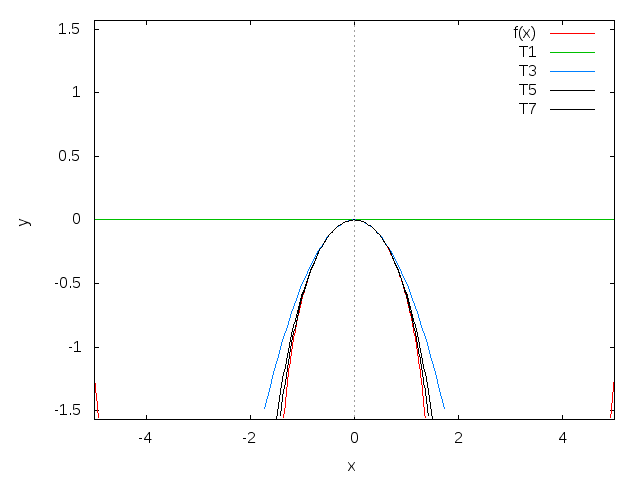
\includegraphics[scale=0.5]{taylorlogcosbien.png}
\end{figure}
  \end{center}\\
  \newpage
  4.- Calcula las aproximaciones de Taylor de la función exp(x)/cos(x), alrededor de x=0.\\
  \begin{verbatim}
  
  f(x):=exp(x)/cos(x);
p(x):= taylor(f(x), x, 0, 1);
t(x):= taylor(f(x), x, 0, 3);
a(x):= taylor(f(x), x, 0, 5);
b(x):= taylor(f(x), x, 0, 7);
plot2d([f(x),p(x), t(x), a(x), b(x)],[x,-3,3],[y,-5,5],\\
  [color,red,green,blue,orange,black], \\
  [legend,"f(x)","T1","T3","T5","T7"]);
tex(p(x));
tex(t(x));
tex(a(x));
tex(b(x));
fortran(p(x));
fortran(t(x));
fortran(a(x));
fortran(b(x));


     \end{verbatim}\\
  
  
 
  \begin{center}
 \begin{figure}[b]
\includegraphics[scale=0.5]{Taylor4.png}
\end{figure}
 \end{center}\\
 \newpage




5.- De la misma forma, ejemplifica la aproximación de Taylor de la función
 (1+x) exp(x), alrededor de x=0.\\
 \begin{verbatim}


 f(x):=(1+x)*exp(x);
p(x):= taylor(f(x), x, 0, 1);
t(x):= taylor(f(x), x, 0, 3);
a(x):= taylor(f(x), x, 0, 5);
b(x):= taylor(f(x), x, 0, 7);
plot2d([f(x),p(x), t(x), a(x), b(x)],[x,-3,3],[y,-5,5],\\
 [color,red,green,blue,orange,black], \\
 [legend,"f(x)","T1","T3","T5","T7"]);
tex(p(x));
tex(t(x));
tex(a(x));
tex(b(x));
fortran(p(x));
fortran(t(x));
fortran(a(x));
fortran(b(x));


 \end{verbatim}




 \begin{center}
 \begin{figure}[b]
\includegraphics[scale=0.5]{Taylor5.png}
\end{figure}
 \end{center}
 \end{document}